\documentclass{article}
\usepackage{graphicx} % Required for inserting images
\usepackage[margin=1in]{geometry}
\usepackage{amsmath}
\usepackage{amsthm}
\usepackage{amssymb}
\usepackage{amsfonts}
\usepackage{enumitem}
\usepackage{verbatim}
\usepackage{xcolor}

\title{Midterm: Report}
\author{Dante Buhl}

\DeclareMathOperator{\cond}{cond}
\DeclareMathOperator{\vecspan}{span}

\begin{document}

\newcommand{\bs}[1]{\boldsymbol{#1}}
\newcommand{\bmp}[1]{\begin{minipage}{#1\textwidth}}
\newcommand{\emp}{\end{minipage}}
\newcommand{\R}{\mathbb{R}}
\newcommand{\C}{\mathbb{C}}
\newcommand{\N}{\mathcal{N}}
\newcommand{\I}{\mathrm{I}}
\newcommand{\K}{\bs{\mathrm{K}}}
\newcommand{\m}{\bs{\mu}_*}
\newcommand{\s}{\bs{\Sigma}_*}
\newcommand{\dt}{\Delta t}
\newcommand{\tr}[1]{\text{Tr}(#1)}
\newcommand{\Tr}[1]{\text{Tr}(#1)}
\newcommand{\hl}[1]{\colorbox{yellow}{#1}}

\maketitle

\section*{Question 1: BVP using Shooting Method and RK4}
\begin{enumerate}[label=\alph*)]

  \item The system can be solved analytically by simply integrating 4 times and
  then solving for the boundary conditions. 
  \begin{align*}
    EI\int\int\int\int \frac{d^4y}{dx^4} dx^4 &= \int\int\int\int x^2 dx^4\\
    EIy(x) &= \frac{x^6}{360} + c_1x^3 + c_2x^2 + c_3x + c_4
  \end{align*}
  We can see very clearly from the boundary conditions at $x=0$ that $c_4=c_3=0$.
  We finish solving for $c_1$ and $c_2$.
  \begin{align*}
    0 = \frac{1}{360} + c_1 + c_2, &\quad 0 = \frac{1}{60} + 3c_1 + 2c_2\\
    c_1 = -\frac{1}{90}, &\quad c_2 = \frac{1}{120}
  \end{align*}
  \begin{align*}
    y(x) = \frac{1}{EI}\left(\frac{x^6}{360} - \frac{x^3}{90} +
    \frac{x^2}{120}\right)
  \end{align*}

  \item \colorbox{yellow}{Determine the Numerical Solution using the shooting method.}


  \item \colorbox{yellow}{Plot the numerical solution obtained with the shooting
  method}

  \item \colorbox{yellow}{Plot the error}

\end{enumerate}


\section*{Question 2: Convergence and Absolute Stability for an Implicit RK3
Method}

\begin{enumerate}[label=\alph*)]

    \item Prove convergence for Implicit RK3.
    \begin{proof}
        Showing convergence is a matter of sending zero-stability and
        consistency. This is a one-step method, so we have the first
        characteristic polynomial, $\rho(z) = z - 1$. This of course satisfies
        the root condition and therefore is zero-stable. Showing consistency 
    \end{proof}

    \item Plot Region of Absolute Statbility (See Fig. 1)
    \begin{figure}[ht]
        \centering 
        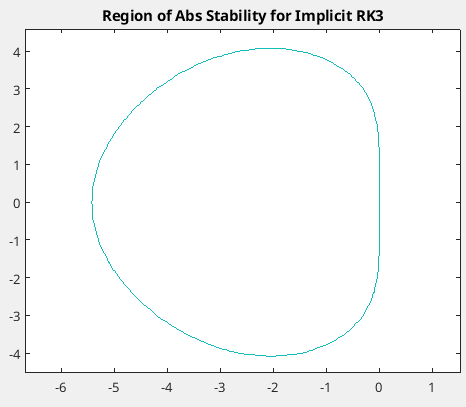
\includegraphics[width=0.5\textwidth]{2.b.AbsStab'.png}
        \caption{Region of Absolute Stability for 2.b.}
    \end{figure}

    \item  
    This problem is solved by plotting the region of absolute stability and
    finding the eignevalues of the matrix B. We notice that since B is an upper
    triangular matrix that its eigenvalues are found on its diagonal. So we have
    that $B$ has all real eigenvalues, $\lambda = \{-1, -2, -4, -16\}$. Next we
    compare to see which eigenvalue is furthest from the region of absolute
    stability. It is evidently the eigenvalue, $\lambda = -16$. So we look at
    the closest point in our region of absolute stability. From the plot we can
    see that the closest point is $\lambda\dt = -5.4199 + 0i$. Therefore we
    have that the largest $\dt$ must be, $\dt \approx 0.338746\ldots$. 

    \item \colorbox{yellow}{Show that this is validated numerically. }

\end{enumerate}

\section*{Question 3: Convergence and Absolute Stability for an LMM}

\begin{align}
    \bs{u}_{k+3} - \frac{1}{3}\left(\bs{u}_{k+2}+\bs{u}_{k+1}+\bs{u}_{k}\right) =
    \frac{\dt}{12}\left[23\bs{f}_{k+2} -2\bs{f}_{k+1} + 3\bs{f}_{k}\right]
\end{align}

\begin{enumerate}[label=\alph*)]

    \item 
    \begin{proof}
        (Zero-Stability)

        We begin this proof first by showing that this LMM is zero-stable. 
        \begin{align*}
            \rho(z) &= z^3 - \frac{1}{3}z^2 - \frac{1}{3}z - \frac{1}{3}\\
            \rho(z) &= (z-1)\left(z^2 + \frac{2}{3}z + \frac{1}{3}\right)\\
            \rho(z) &= (z-1)\left(z - \frac{-\frac{2}{3} \pm \sqrt{\frac{4}{9} -
            \frac{4}{3}}}{2}\right)\\
            \rho(z) &= (z-1)\left(z + \frac{1 \pm i\sqrt{2}}{3}\right)
        \end{align*}
        These are the three complex roots of the characteristic polynomial. We
        now simply must check if all three are within or on the boundary of the
        unit disk. 
        \begin{align*}
            |1| = 1 \le 1, \quad \left|\frac{1 \pm i\sqrt{2}}{3}\right| =
            \frac{1}{9} + \frac{2}{9} = \frac{1}{3} \le 1
        \end{align*}
        As I have just shown, in fact all three roots of the first
        characteristic polynomial fall within the unit disk or on the boundary,
        thus we have that this LMM is zero-stable. 

        (Consistency) 

        We we will look at the consistency of this LMM. We look at the
        definition of truncation error in our system. 
        \begin{align*}
            \bs{y}_{k+3} - \frac{1}{3}(\bs{y}_{k+2} + \bs{y}_{k+1} + \bs{y}_{k}) &=
            \frac{\dt}{12}[\dot{\bs{y}}_{k+2} - 2\dot{\bs{y}}_{k+1} + 3\dot{\bs{y}}_{k}] + \dt
            \tau_{k+3}
        \end{align*}
        We look at the taylor expansions for several points in the LMM. 
        \begin{align*}
            \bs{y}_{k} &= \bs{y}_{k+3} - 3\dt \dot{\bs{y}}_{k} - \frac{9}{2}\dt^2\ddot{\bs{y}}_{k} -
            \frac{27}{6}\dt^3\dddot{\bs{y}}_{k} - \frac{81}{24}\dt^4\ddddot{\bs{y}}_{k} +
            h.o.t.\\
            \bs{y}_{k+1} &= \bs{y}_{k+3} - 2\dt \dot{\bs{y}}_{k+1} - \frac{4}{2}\dt^2\ddot{\bs{y}}_{k+1} -
            \frac{8}{6}\dt^3\dddot{\bs{y}}_{k+1} - \frac{16}{24}\dt^4\ddddot{\bs{y}}_{k+1} +
            h.o.t.\\
            \bs{y}_{k+2} &= \bs{y}_{k+3} - \dt \dot{\bs{y}}_{k+2} - \frac{1}{2}\dt^2\ddot{\bs{y}}_{k+2} -
            \frac{1}{6}\dt^3\dddot{\bs{y}}_{k+2} - \frac{1}{24}\dt^4\ddddot{\bs{y}}_{k+2}+
            h.o.t.
        \end{align*}
        \begin{align*}
            \tau_{k+3} &= \frac{\bs{y}_{k+3} - \frac{1}{3}(\bs{y}_{k+2} +
            \bs{y}_{k+1} + \bs{y}_{k})}{\dt} - \frac{1}{12}[\dot{\bs{y}}_{k+2} 
            - 2\dot{\bs{y}}_{k+1} + 3\dot{\bs{y}}_{k}]\\\\
            \tau_{k+3} &= -\frac{\bs{y}_{k+3} - 3\dt \dot{\bs{y}}_{k} - \frac{9}{2}\dt^2\ddot{\bs{y}}_{k} -
            \frac{27}{6}\dt^3\dddot{\bs{y}}_{k} - \frac{81}{24}\dt^4\ddddot{\bs{y}}_{k} +
            h.o.t.}{3\dt}\\\\
            &- \frac{\bs{y}_{k+3} - 2\dt \dot{\bs{y}}_{k+1} - \frac{4}{2}\dt^2\ddot{\bs{y}}_{k+1} -
            \frac{8}{6}\dt^3\dddot{\bs{y}}_{k+1} - \frac{16}{24}\dt^4\ddddot{\bs{y}}_{k+1} +
            h.o.t.}{3\dt}\\\\
            &-\frac{\bs{y}_{k+3} - \dt \dot{\bs{y}}_{k+2} - \frac{1}{2}\dt^2\ddot{\bs{y}}_{k+2} -
            \frac{1}{6}\dt^3\dddot{\bs{y}}_{k+2} - \frac{1}{24}\dt^4\ddddot{\bs{y}}_{k+2}+
            h.o.t.}{3\dt} \\\\
            &+ \frac{\bs{y}_{k+3}}{\dt} - \frac{1}{12}[23\dot{\bs{y}}_{k+2} -
            2\dot{\bs{y}}_{k+1} + 3\dot{\bs{y}}_{k}] \\\\
            \tau_{k+3} &= \frac{9\dot{\bs{y}}_k + 10\dot{\bs{y}}_{k+1}
            -19\dot{\bs{y}}_{k+2}}{12} + h.o.t
        \end{align*}
    \end{proof}

    \item Absolute Stability and A-Stability

    We can plot the region of absolute stability for this LMM. We have the first
    and second characterstic polynomials are the following. 
    \begin{align*}
        \rho(z) = z^3 - \frac{1}{3}\left(z^2 + z + 1\right), &\quad \sigma(z) =
        \frac{1}{12}\left(23z^2 - 2z + 3\right)\\
        \frac{\rho(z)}{\sigma(z)} = \lambda \dt 
    \end{align*}
    We can then plot this by evaluating $\frac{\rho(z)}{\sigma(z)}$ with
    $z=e^{i\theta}$ and plotting in the complex plane. 
    \begin{figure}[h]
        \centering 
        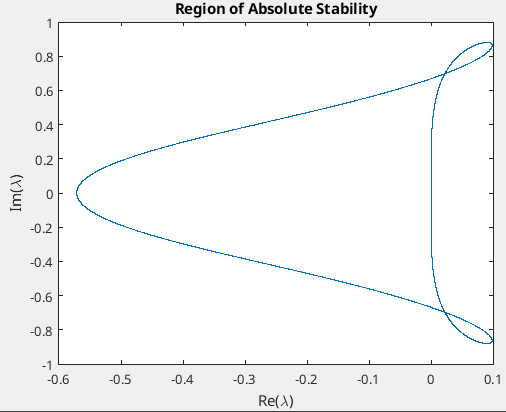
\includegraphics[width=0.5\textwidth]{3.b.AbsStab.png}
        \caption{Region of Absolute Stability for 3.b}
    \end{figure}
    We can see from this plot that this LMM is certainly not A-Stable. The
    reason being that the region of absolute stability is only conditionally
    absolutely stable. This is seen in the plot which clearly illurstrates the
    region of absolute stability including only a small subset of $\C^-$. 
    

\end{enumerate}

\end{document}
